% !TEX root = ../../../main.tex
% !TEX encoding = UTF-8 Unicode
% !TEX encoding = UTF-8

\subsection{Zeitplanung - BB}
% \textit{Autor: Benedikt Buchner}

Neben der Einschätzung der zu erwarteten Kosten soll der zeitliche Ablauf der einzelnen Projektkomponenten beleuchtet werden. Die aufsummierte Dauer der einzelnen Komponenten ergibt dann den gesamten zeitlichen Aufwand Projekts. Zur zeitlichen Planung der erforderlichen Schritte, sowie der Ablaufplanung einzelner Arbeitspakete werden Gantt-Diagramme eingesetzt. Die Anwendung eines solchen Gantt-Diagramms stellt das erste Kapitel dieses Abschnitts dar. Die Einhaltung der zuvor definierten Meilensteine und Arbeitsschritte wird dabei anhand der Meilensteintrendanalyse durchgeführt. Wie die Meilensteintrendanalyse zur Überwachung der Projektmodule eingesetzt werden soll wird im zweiten Teil dieses Kapitels erklärt.

\subsubsection{Gantt-Diagramm}
Zur Erstellung eines Gantt-Diagramms ist es wichtig, zunächst eine Aktivitätenliste zu erstellen, die durch das Zerlegen von Arbeitspaketen generiert wird. Eine Möglichkeit diese Arbeitspakete zu ermitteln besteht im Erstellen eines Projektstrukturplans. Eine Aktivität erhält dabei, neben Metainformationen, wie einer eindeutigen Nummer und der Person der diese Aktivität zugwiesen wird, für die zeitliche Planung entscheidende Parameter wie der genauen Dauer dieser Aktivität und einer möglichen Wartezeit die vor oder nach dem Abarbeiten selbiger eintritt.\footnote{\cite{kraus_projekt_2010}}  Da das Schätzen der benötigten Zeit zur Bearbeitung einer Aktivität im Kontext dieses Projekts stark von Erfahrungen abhängt, sollen hierzu Experten bezüglich dieser Erfahrungswerte befragt werden.

Die Darstellung eines Gantt-Diagramms unterliegt keinen gestalterischen Vorgaben oder Richtlinien und sind für alle Ebenen der Planung einsetzbar. Jede Aktivität muss lediglich durch einen Balken dargestellt werden, dessen Länge proportional zu der Dauer der Aktivität ist.\footnote{\cite{jakoby_intensivtraining_2015}}

Ein großer Vorteil dieser Diagrammart ist die Übersichtlichkeit, da es durch den Aufbau des Diagramms möglich ist, auf einen Blick zu erkennen wann welche Aktivität begonnen werden und wann diese beendet sein muss. Ein Nachteil ist die Tatsache, dass mögliche Abhängigkeiten nicht aufgezeigt werden können.\footnote{\cite{kraus_projekt_2010}}

Die zuvor aus den Aufgabenpaketen ermittelten Aktivitäten werden also in das Gantt-Diagramm übertragen und mit entsprechenden Balken versehen. Dies wird in Abbildung \ref{fig_beispiel_gantt_diagramm} verdeutlicht:

\begin{figure}[h!]
	\centering
	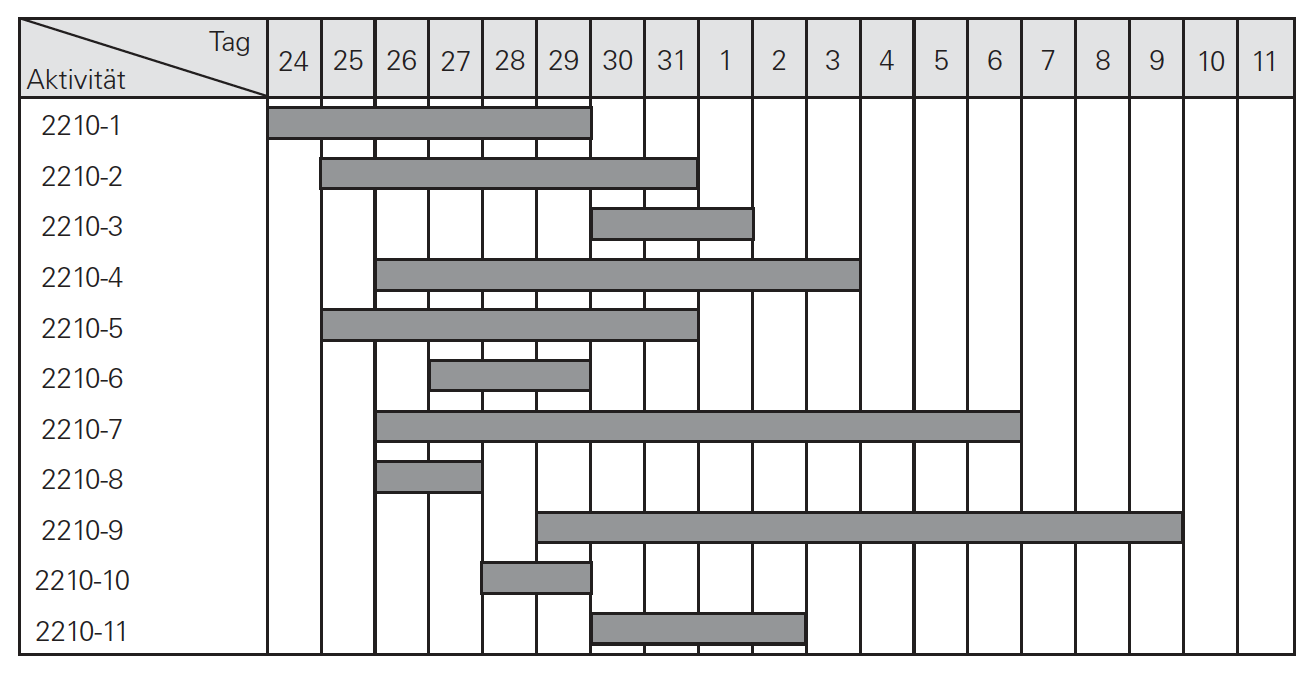
\includegraphics[width=\textwidth]
	{kapitel/gruppe4_2/bilder/beispiel_gantt_diagramm}
	\caption{Beispiel eines Gantt-Diagramms}
	\label{fig_beispiel_gantt_diagramm}
\end{figure}

Die Aktivitäten werden, wie das Beispiel zeigt, vertikal erfasst. Die horizontale Achse bildet den zeitlichen Ablauf ab. Sie ist frei definierbare Zeiteinheiten, hier Tage, unterteilt. Den einzelnen Aktivitäten wurde in Abhängigkeit ihrer Dauer ein jeweils entsprechend langer Balken zugeordnet.

Es gilt zu beachten, dass für jede Komponente die innerhalb des Projekts umgesetzt werden soll, ein solches Diagramm erstellt wird. Damit wird der hohen Modularität des Projekts Rechnung getragen und eine entsprechend agile Priorisierung der umzusetzenden Komponenten ist möglich. Die Reihenfolge der Umsetzung ist somit frei wählbar, ohne dabei die Möglichkeit einer zeitlichen Planung bei der Umsetzung innerhalb Komponente zu verlieren.

\subsubsection{Meilensteintrendanalyse}
Die Meilensteintrendanalyse (MTA) ist ein wichtiges und dabei einfach anzuwendendes Werkzeug zur Überwachung essentieller Projekttermine. In diesem Zusammenhang werden Projekttermine auch Meilensteine genannt. Die MTA liefert dabei zwei grundlegende Informationen: Einerseits liefert sie einen Überblick über die Entwicklung zukünftiger Termine, andererseits lässt sich anhand dieser Entwicklung die Stabilität der Terminprognosen erkennen.\footnote{\cite{gadatsch_masterkurs_2014}}

Abbildung \ref{fig_MTA_diagramme} zeigt exemplarisch den Aufbau eines MTA-Diagramms:
\begin{figure}[h!]
	\centering
	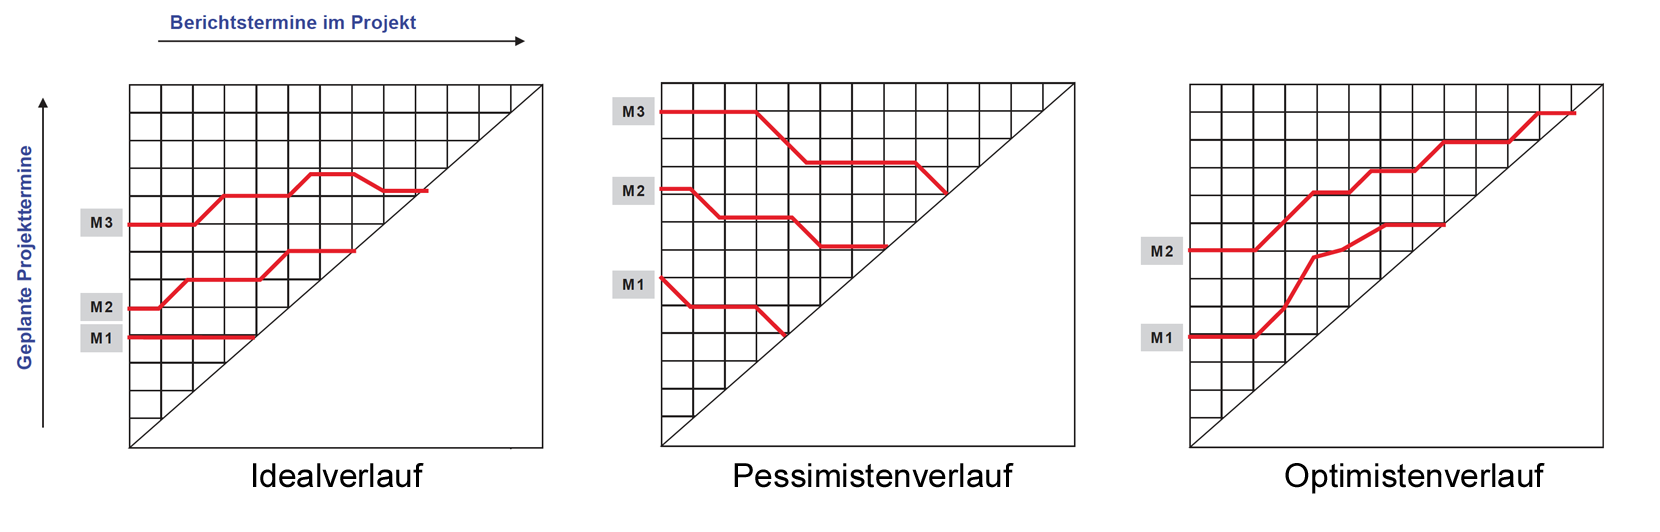
\includegraphics{kapitel/gruppe4_2/bilder/mta_diagramme}
	\caption{Mögliche Ausprägungen der MTA Diagramme}
	\label{fig_MTA_diagramme}
\end{figure}

In der Abbildung \ref{fig_MTA_diagramme} ist zu erkennen, dass ein MTA-Diagramm zwei Dimensionen besitzt. Auf der horizontalen Achse werden die Berichtstermine in vorher vereinbarten und regelmäßigen Abständen aufgetragen. Die vertikale Achse ist mit den geplanten Projekterminen (Meilensteinen) beschriftet. Die Schnittstellen der Achsen geben das aktuelle, möglicherweise korrigierte Fälligkeitsdatum des Meilensteins zum Zeitpunkt des Berichts an. In jedem Bericht müssen die Meilensteintermine neu bewertet werden. Dabei ist es irrelevant ob der Termin sich nach hinten verschiebt, der Termin dem der letzten Beurteilung entspricht oder das geplante Datum unterschritten werden kann. Die Ergebnisse dieser Beurteilungen werden in dem Diagramm eingetragen, woraus sich im Laufe des Projekts Kurven ergeben. Diese Kurven entsprechen in der Regel einem der drei typischen Verläufe. Fallende Kurven zeigen, dass die Termine initial zu pessimistisch geschätzt wurden und häufig nach unten korrigiert werden mussten. Steigende Kurven bedeuten hingegen, dass Termine zu optimistisch geschätzt wurden. Die weitestgehend gerade verlaufenden Kurven stellen entsprechend den Idealverlauf dar.\footnote{\cite{gadatsch_masterkurs_2014}}
